%pdflatex --shell-escape scap_benchmark_dl_training
%biber scap_benchmark_dl_training 

\PassOptionsToPackage{hyphens}{url}
\documentclass[compress,aspectratio=169]{beamer}

\usepackage[official]{eurosym}
\usepackage{multirow}
\setlength{\marginparwidth}{2cm}
\usepackage{todonotes}
\presetkeys{todonotes}{inline}{}
\usepackage[style=verbose,backend=biber,style=authoryear, citestyle=authoryear ]{biblatex}
\setbeamertemplate{bibliography item}{\insertbiblabel} % Ensure that cite labels appear in references section
\addbibresource{ref.bib}
\usepackage{./assets/beamerthemeGoettingen} % make sure the theme file is on this path
\graphicspath{{../}{./assets/}}
\usepackage{caption}
\usepackage{booktabs}
\usepackage[normalem]{ulem}

\hypersetup{
    colorlinks,
    citecolor=black,
}

\newcommand{\source}[1]{\par\begin{textblock*}{6cm}(1cm,8cm)
    \begin{beamercolorbox}[wd=\paperwidth,ht=0.5cm,right]{framesource}
        \usebeamerfont{framesource}\usebeamercolor[fg]{framesource} \centering\tiny {#1}
    \end{beamercolorbox}
\end{textblock*}}


% listing / code
\usepackage{minted}
\usemintedstyle{tango}
% Box listing / code
\usepackage{tcolorbox}

% Box listing / code style 
% These options will be applied to all `tcolorboxes`
\tcbset{%
    noparskip,
    colback=gray!5, %background color of the box
    colframe=gray!20, %color of frame and title background
    coltext=black, %color of body text
    coltitle=black, %color of title text 
    fonttitle=\tiny,
    alerted/.style={coltitle=red, 
                     colframe=gray!40},
    example/.style={coltitle=black, 
                     colframe=green!20,             
                     colback=green!5},
    }

\lstset{literate=%
    {Ö}{{\"O}}1
    {Ä}{{\"A}}1
    {Ü}{{\"U}}1
    {ß}{{\ss}}1
    {ü}{{\"u}}1
    {ä}{{\"a}}1
    {ö}{{\"o}}1
    {~}{{\textasciitilde}}1
}

\usepackage{csquotes} % For \enqoute{}
\usepackage{hyperref}

% --- document configuration ---
\newcommand{\mytitle}{Getting started with profiling PyTorch - PointNet}     
% Leave empty for no subtitle
\newcommand{\mysubtitle}{State of the art and plan for Scalable Computing Systems and Applications in AI, Big Data and HPC}   
\newcommand{\myauthor}{Hauke Kirchner}
\newcommand{\myauthorurl}{\href{http://www.overleaf.com}{Something 
Linky}}
\newcommand{\myvenue}{Göttingen}
% For example, use \today
\newcommand{\mydate}{24.11.2022}
% For example, Institute for Computer Science / GWDG
\newcommand{\myinstitute}{GWDG - AG Computing}
% Leave empty for no footer image
\newcommand{\myfooterimage}{}           
\newcommand{\mygrouplogo}{}
% Images must be enabled manually under title page \titleLogo
% Adjust position and width manually for fewer images
\newcommand{\mytitleimageone}{}         
\newcommand{\mytitleimagetwo}{}        
\newcommand{\mytitleimagethree}{}

% --- title page ---
\title{\Large \mytitle}
\venue{\myvenue}
\date{\mydate}
\subtitle{\mysubtitle}
%\authorURL{\myauthorurl}
\author{{\myauthor}}
\authorFooter{\myauthor \hspace{0.3cm} \includegraphics[height=1em]{\myfooterimage}}
\institute{\myinstitute}
\groupLogo{\includegraphics[width=2cm]{\mygrouplogo}}
\titleLogo{
%\includegraphics[height=2.7cm]{\mytitleimageone}
%\includegraphics[height=2.7cm]{\mytitleimagetwo}
%\includegraphics[height=2.7cm]{\mytitleimagethree}
}

\setbeamertemplate{footline}[text line]{
\begin{beamercolorbox}[sep=0.5em,wd=\paperwidth,leftskip=0.2cm,rightskip=0.1cm]{footlinecolor}
\myauthor \hfill \insertVenue \hfill \insertframenumber\,/\,\ref{pg:lastpage}
\end{beamercolorbox}
}

\begin{document}

\begin{frame}[plain]
	\titlepage
\end{frame}

\begin{frame}[t]{Table of contents}
  \tableofcontents[subsectionstyle=hide/hide]
\end{frame}

\section{PyTorch Profiler: Optimized data loading strategy}

\begin{frame}{Training setup}
\begin{itemize}
    \item number of trees for training: 8000 (740 GB)
    \vspace{1em}
    \item number of trees for testing: 2000 (191GB)
    \vspace{1em}
    \item trained for 15 epochs
\end{itemize}
\end{frame}


\begin{frame}{Long training times for original workflow}
    \begin{center}
    \begin{figure}
        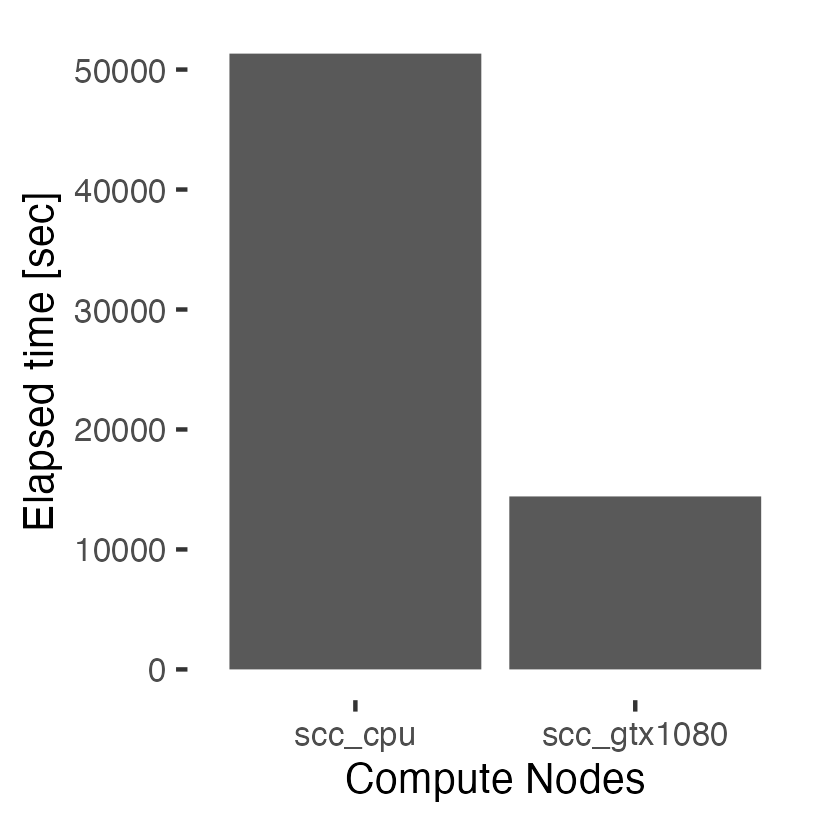
\includegraphics[width=0.5\textwidth]{./assets/sacct_barplot_by_nodes_profiler-torch_sample-points}
    \end{figure}
    \end{center}
\end{frame}

\begin{frame}{Trying to use the PyTorch Profiler to find the bottleneck}
    \vspace{-1em}
    \begin{center}
    \begin{figure}
        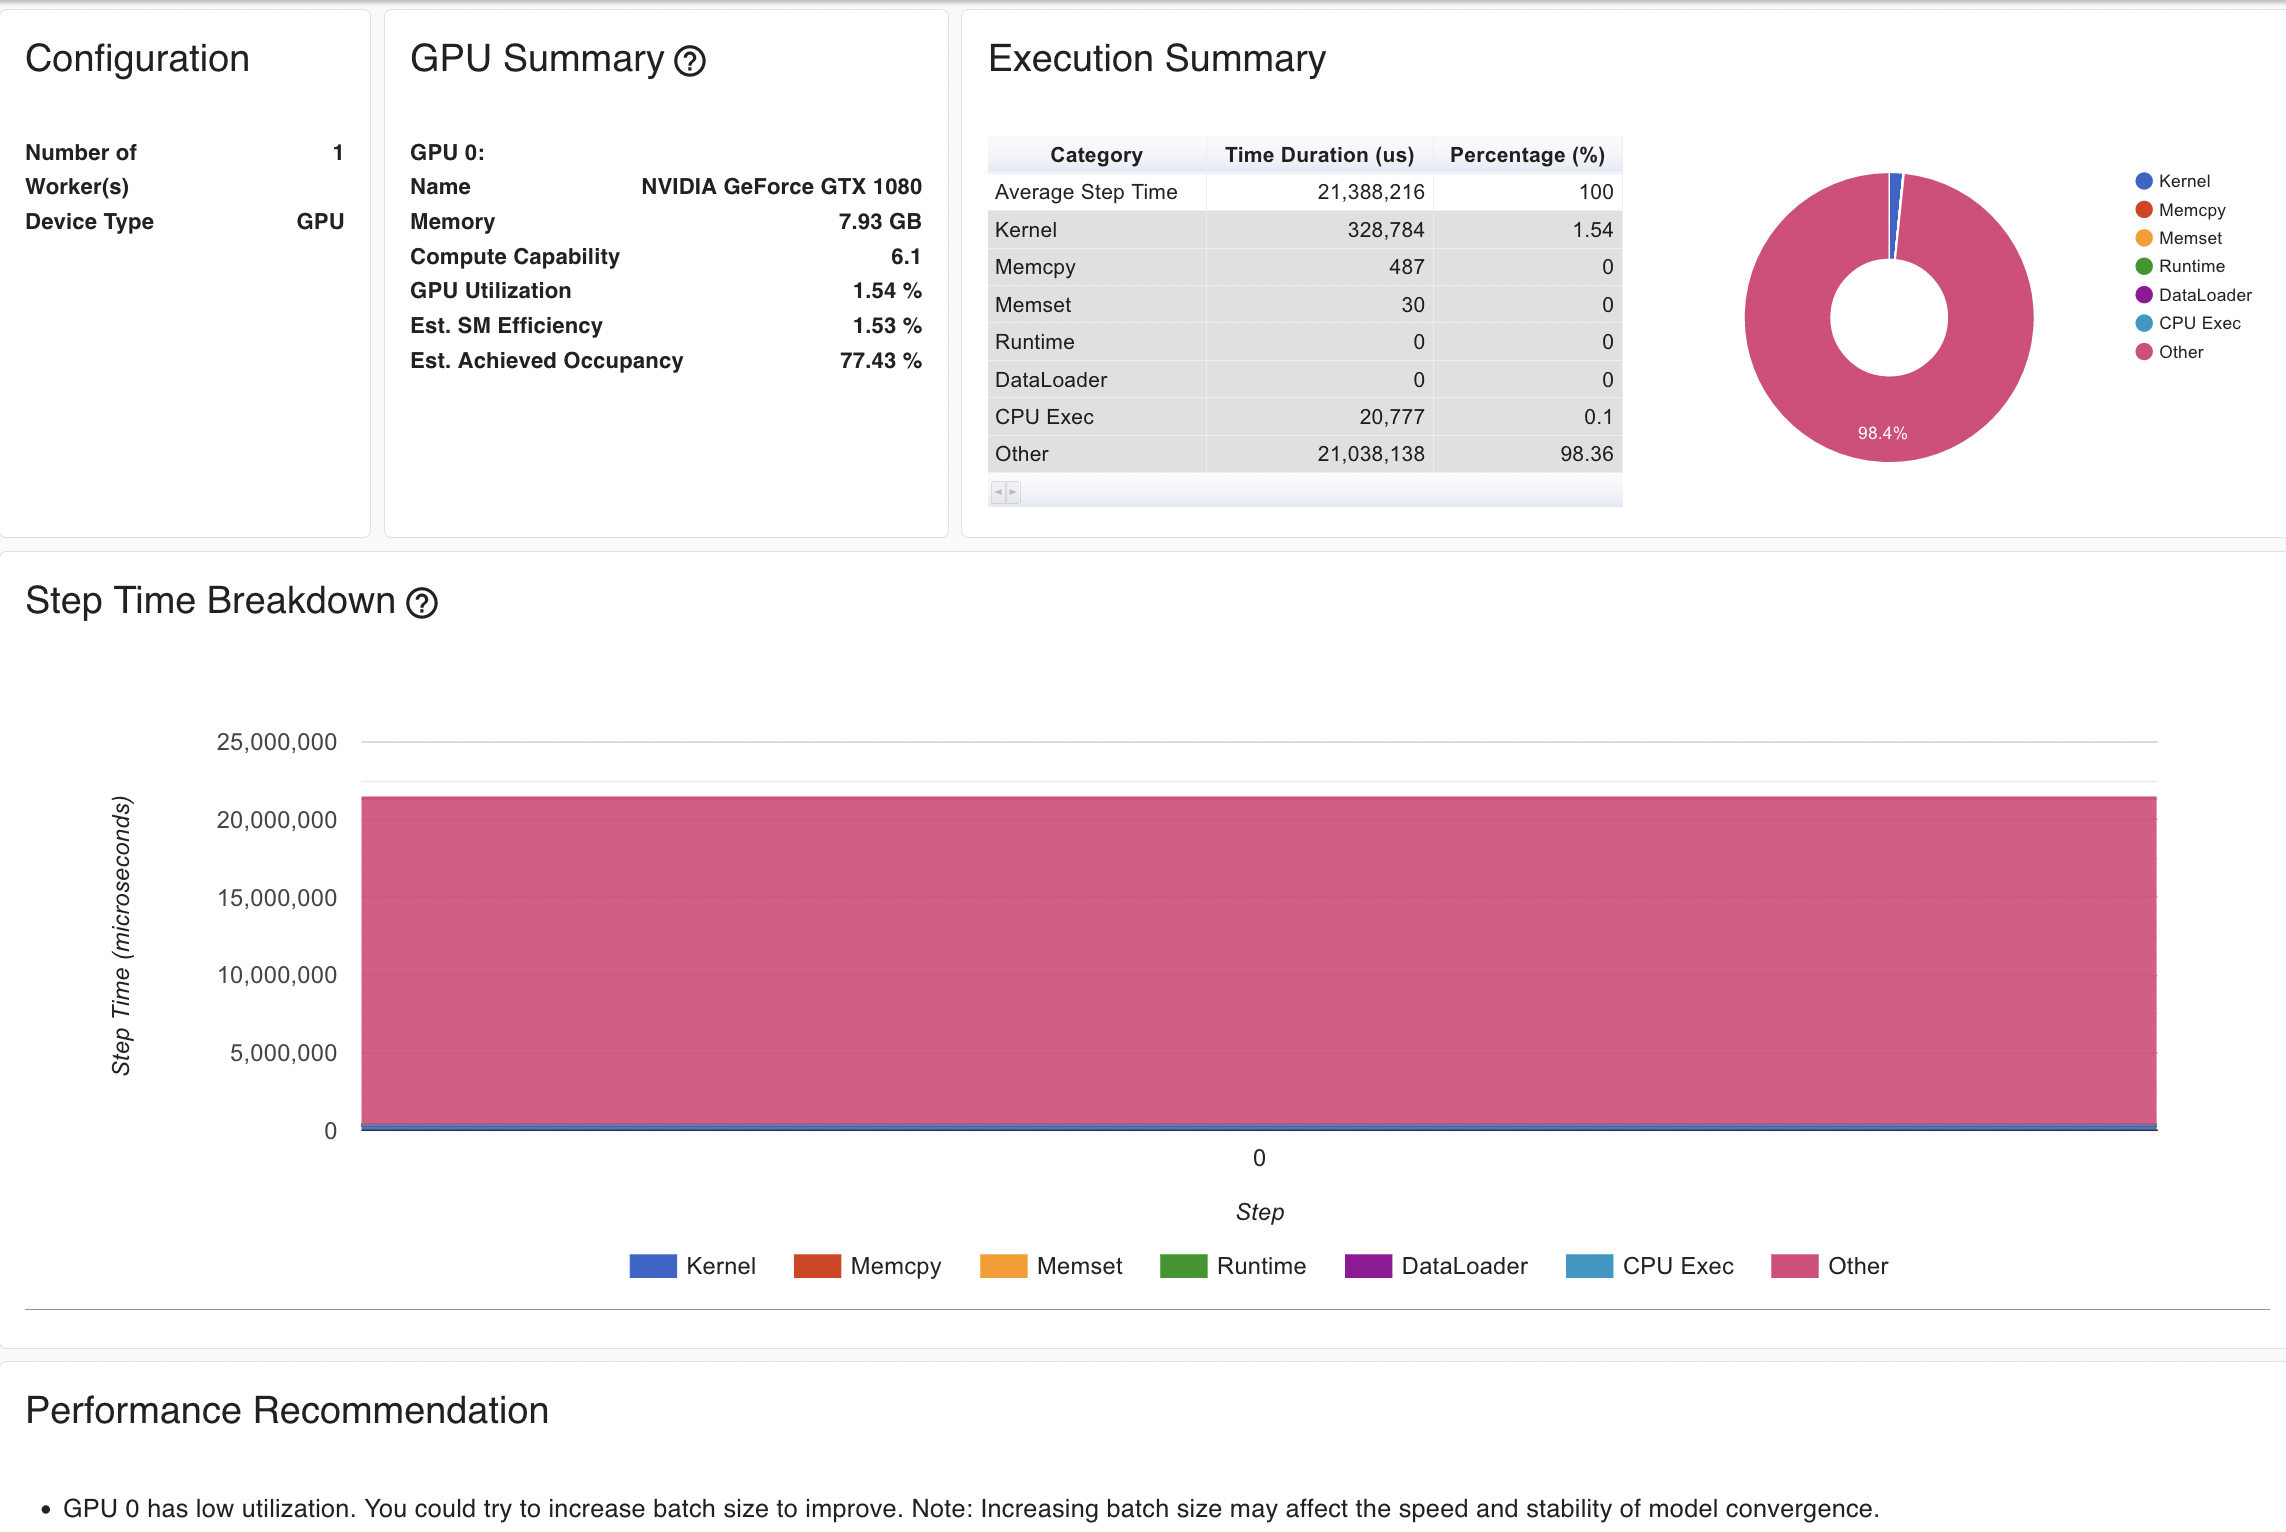
\includegraphics[width=0.75\textwidth]{./assets/scap_gtx1080_profiler-torch_sample-points_14650750}
    \end{figure}
    \end{center}
\end{frame}

\begin{frame}{Trying to use the PyTorch Profiler to find the bottleneck}
    \vspace{-1em}
    \begin{center}
    \begin{figure}
        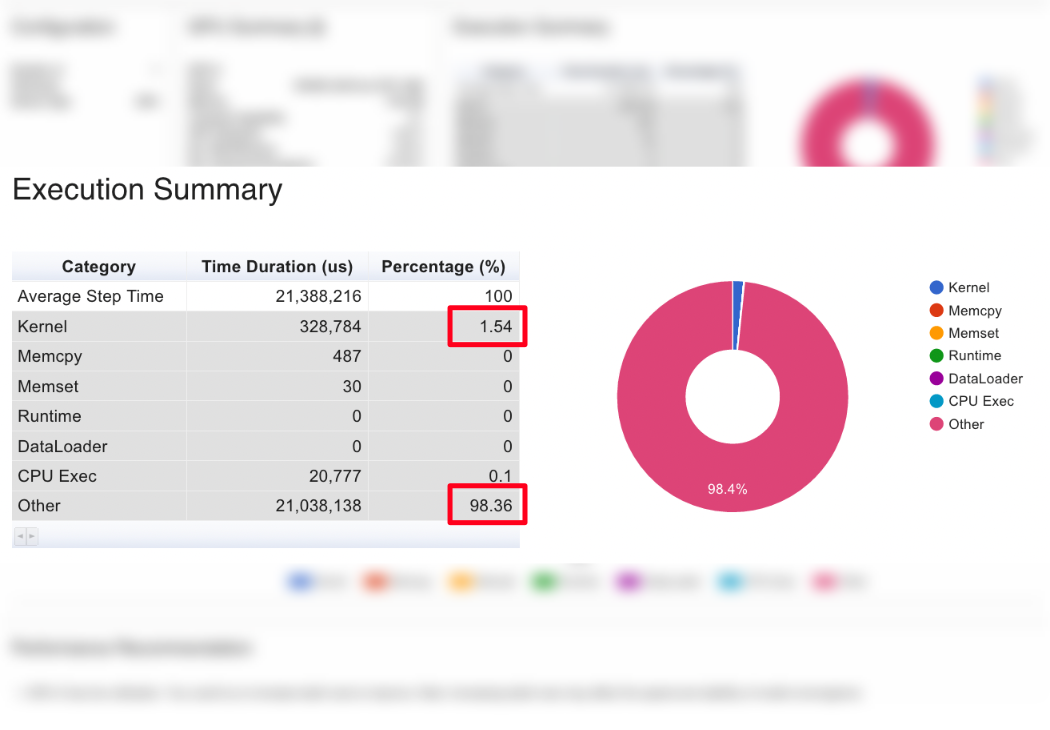
\includegraphics[width=0.9\textwidth]{./assets/scap_gtx1080_profiler-torch_sample-points_14650750_execution-time}
    \end{figure}
    \end{center}
\end{frame}

\begin{frame}{Trace View: Laspy with raw lidar data}
    \vspace{-1em}
\begin{center}
    \begin{figure}
        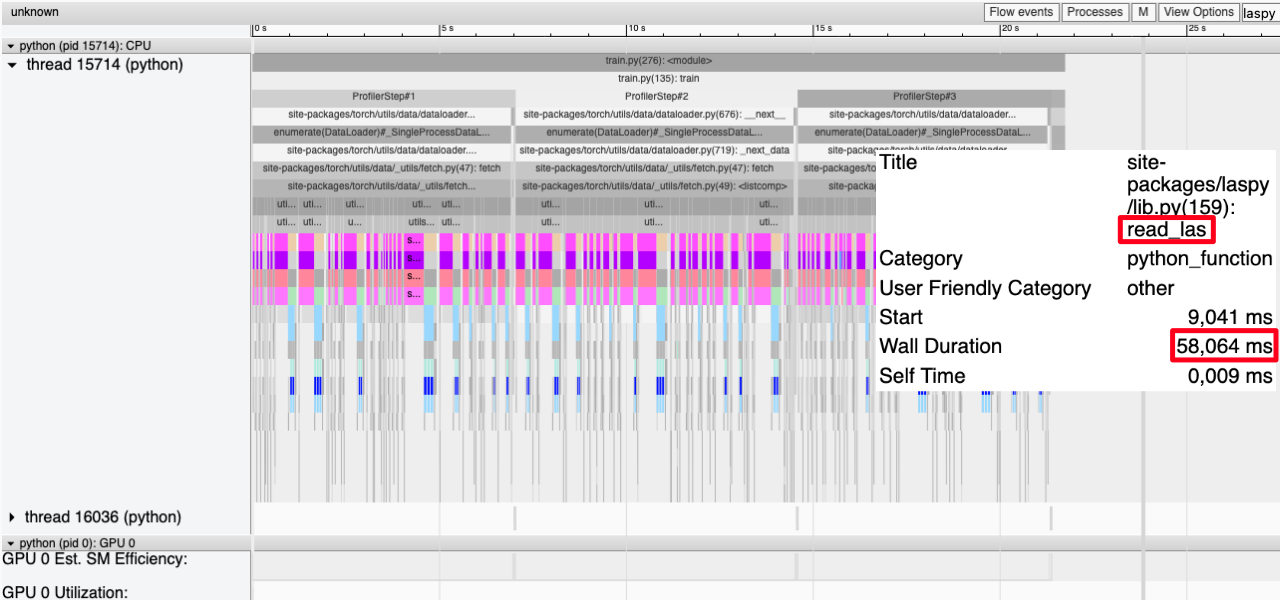
\includegraphics[width=1\textwidth]{./assets/scap_gtx1080_profiler-torch_sample-points_14650750_trace-view-laspy}
    \end{figure}
    \end{center}
\end{frame}

\begin{frame}{Identification of the bottleneck}

\begin{columns}
        \begin{column}{0.5\textwidth}
            \centering
            \vspace{-1em}
            \begin{figure}
            
\includegraphics[width=0.7\textwidth]{./assets/icon_question}
            \end{figure}
        \end{column}
        \begin{column}{0.5\textwidth}
            \begin{itemize}
                \item bottleneck
                \begin{itemize}
                    \item data loading and \\sampling process
                \end{itemize}
                \item solution
                    \begin{itemize}
                        \item sample points before training
                    \end{itemize}
                \vspace{2em}
                \hline
                \vspace{2em}
                \item expert knowledge about the workflow and the profiler required
            \end{itemize}
        \end{column}
    \end{columns}

\end{frame}

\begin{frame}{Effect of point sampling strategies on walltime}
    \vspace{-1em}
    \begin{center}
    \begin{figure}
        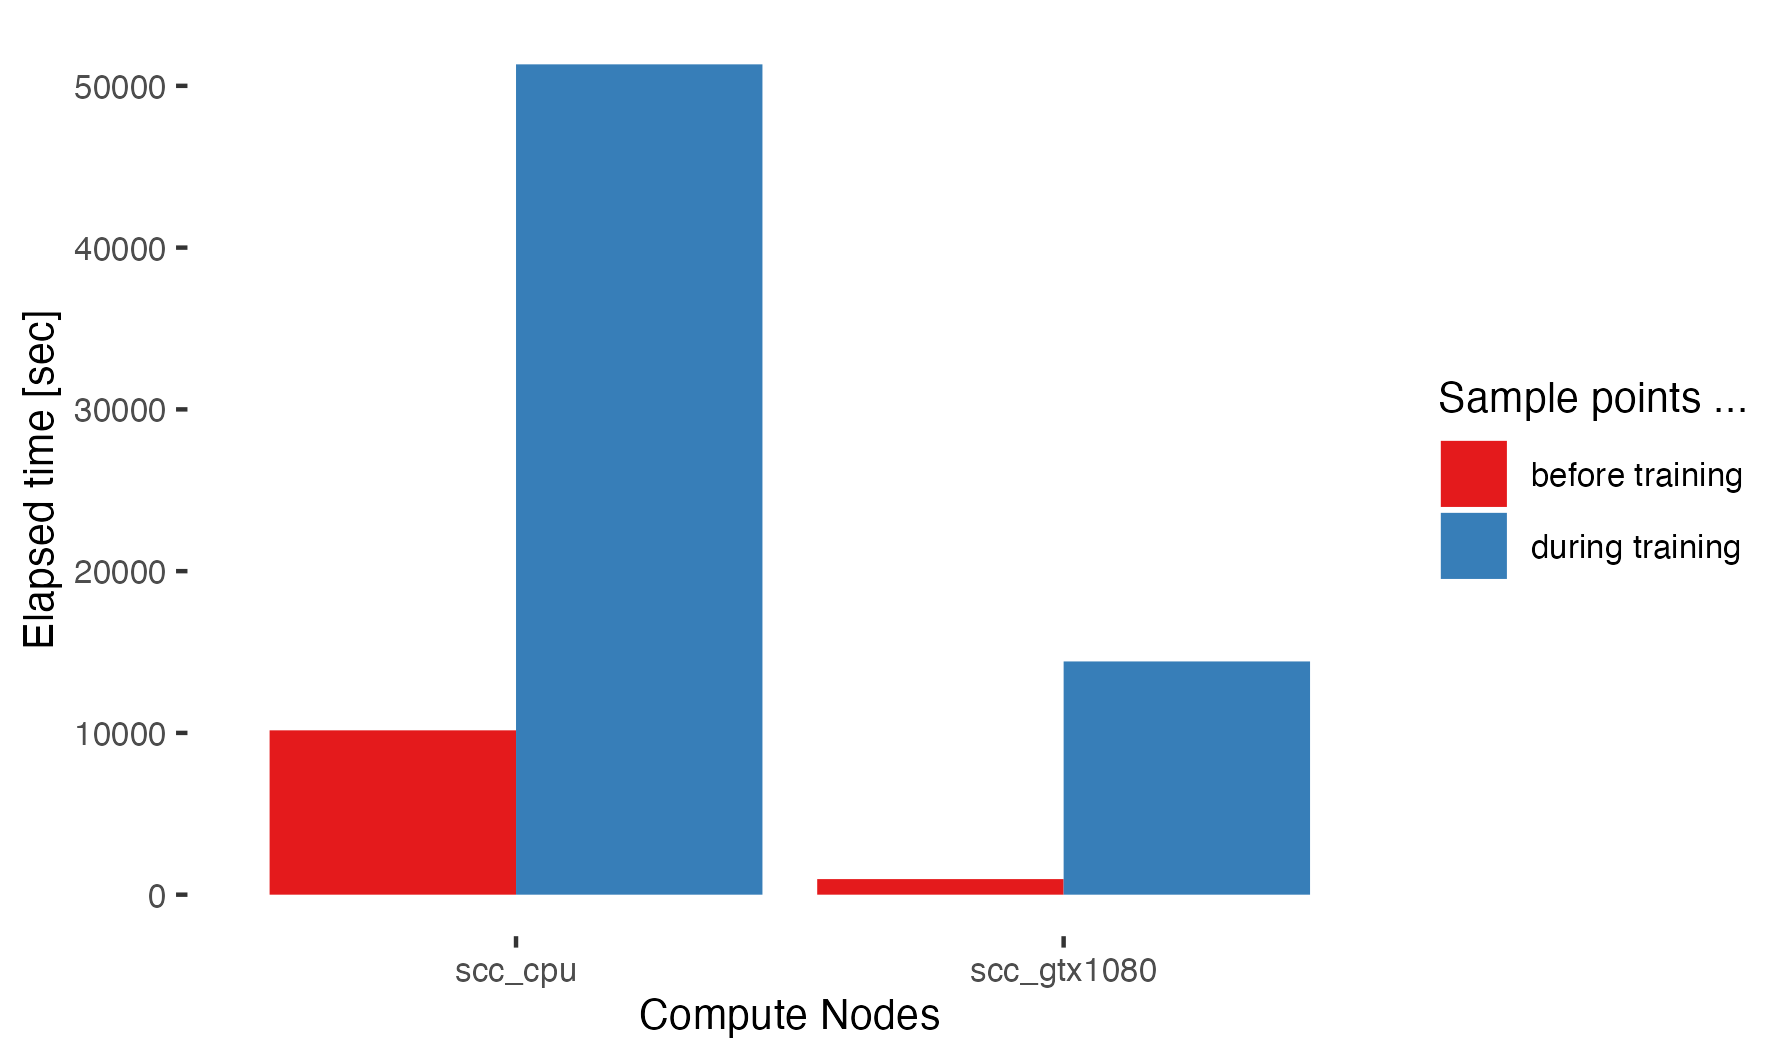
\includegraphics[width=0.85\textwidth]{./assets/sacct_barplot_by_nodes_sample-points-effect}
    \end{figure}
    \end{center}
\end{frame}

\end{frame}

\begin{frame}{Trace View: Laspy with presampled lidar data}
    \vspace{-1em}
\begin{center}
    \begin{figure}
        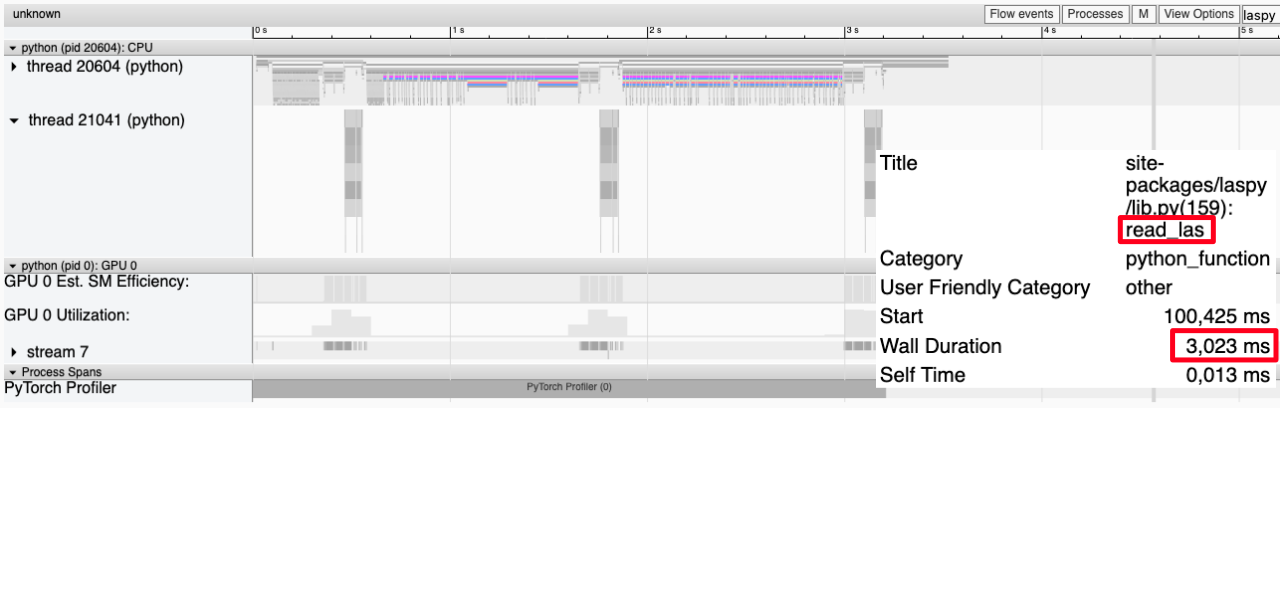
\includegraphics[width=1\textwidth]{./assets/scap_gtx1080_profiler-torch_batch-size-64_14650758_trace-view-laspy}
    \end{figure}
    \end{center}
\end{frame}

\begin{frame}{Training setup - improved}
\begin{itemize}
    \item number of trees for training: 8000 (\sout{740 GB} 434 MB)
    \vspace{1em}
    \item number of trees for testing: 2000 (\sout{191 GB} 109MB)
    \vspace{1em}
    \item trained for 15 epochs
    \vspace{2em}
    \hline
    \vspace{2em}
    \item[$\rightarrow$] reduced hardware usage (energy + money savings)
    \item[$\rightarrow$] more variations of hardware and tools can be tested
\end{itemize}
\end{frame}

\section{PyTorch Profiler: Performance Recommendation}
%\sectionIntroHidden % Show an outline of the current section with hidden subsections
%\sectionIntro % Show an outline of the current section with subsections

\begin{frame}{PyTorch Profiler: Views}
\begin{itemize}
    \item \textbf{Overview}
    \item Operator View
    \item GPU Kernel View
    \item \textbf{Trace View}
    \item Memory View
    \item Module View
\end{itemize}
\end{frame}

\begin{frame}{Overview}
    \vspace{-1em}
\begin{center}
    \begin{figure}
        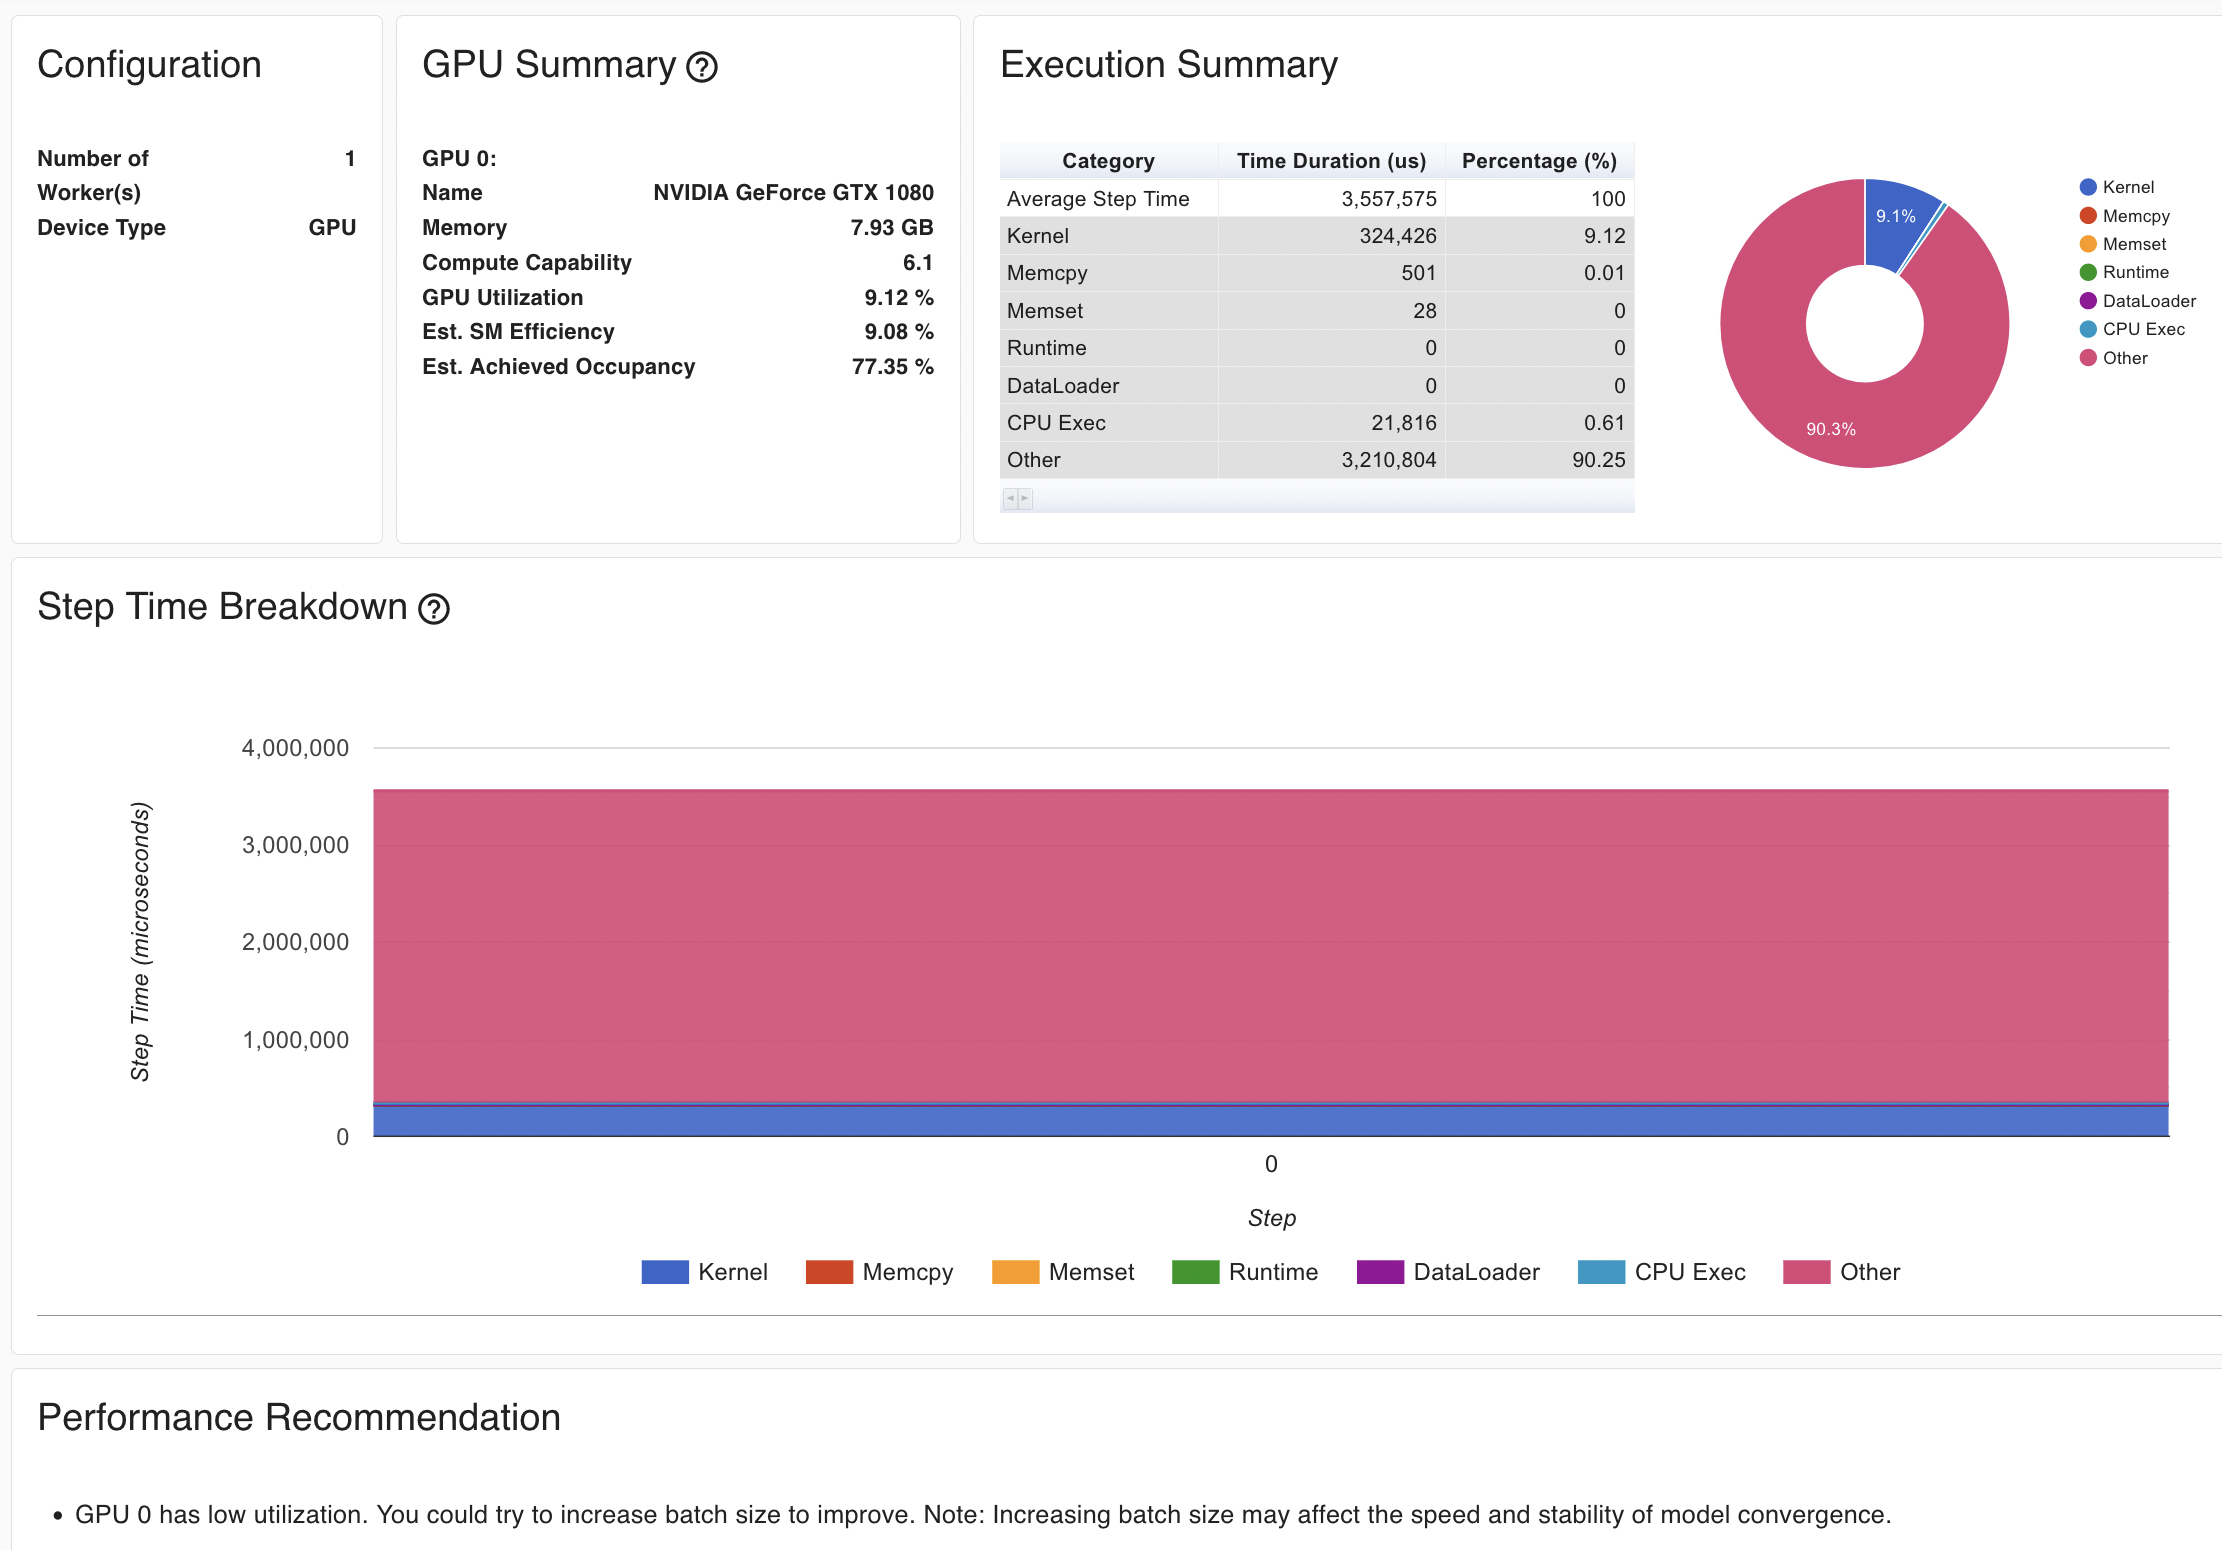
\includegraphics[width=0.7\textwidth]{./assets/scap_gtx1080_profiler-torch_14650076}
    \end{figure}
\end{center}

\end{frame}

\begin{frame}{Performance Recommendation}

\begin{center}
    \begin{figure}
        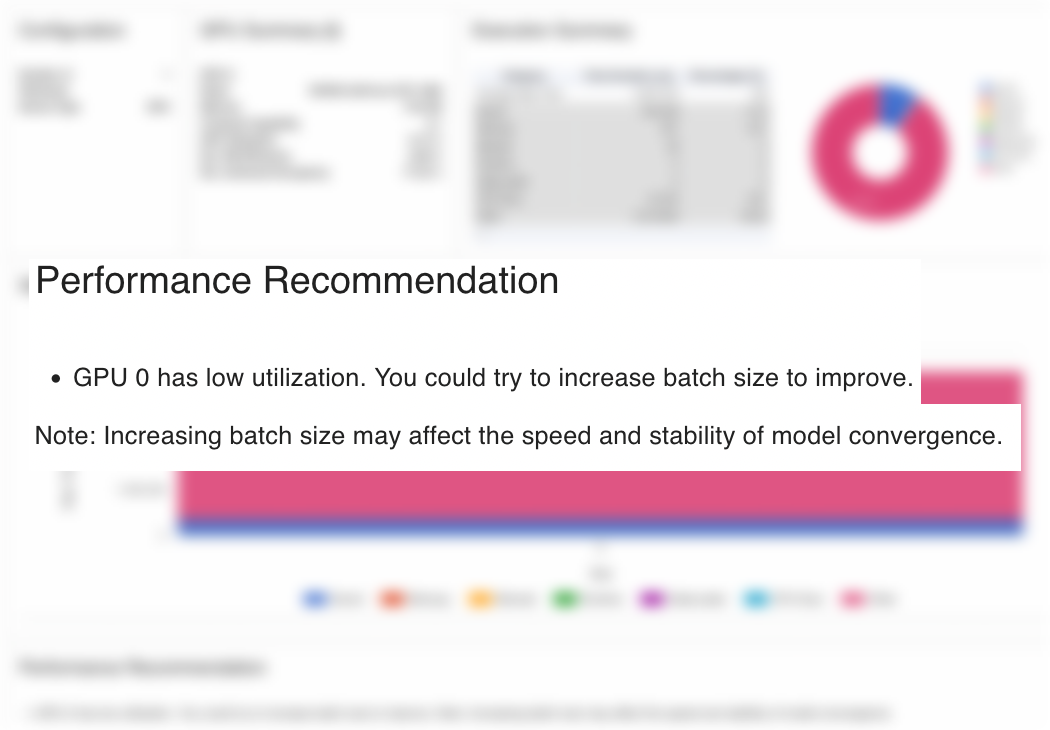
\includegraphics[width=0.7\textwidth]{./assets/scap_gtx1080_profiler-torch_14650076_zoom}
    \end{figure}
\end{center}

\end{frame}


\begin{frame}{Effect of increasing the batch size}
    \vspace{-0.5em}
\begin{center}
    \begin{figure}
        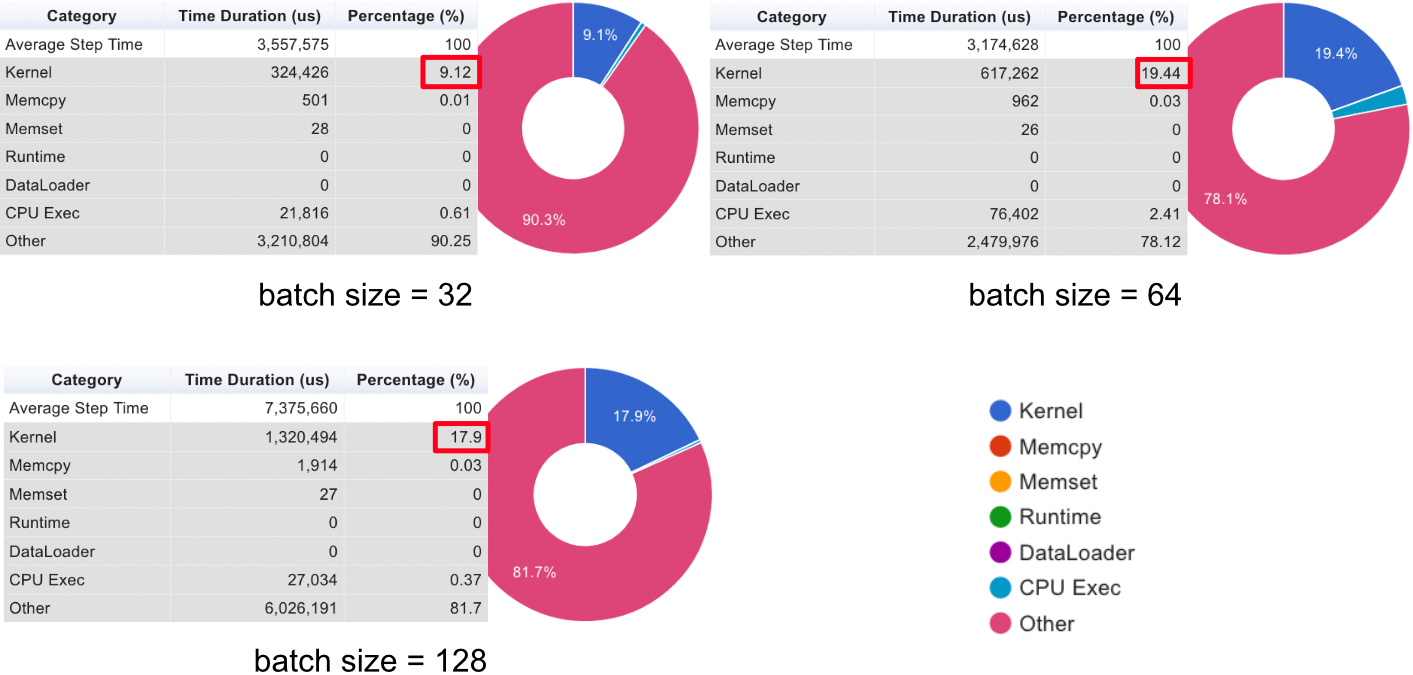
\includegraphics[width=1\textwidth]{./assets/scap_gtx1080_profiler-torch_comparison-batch-size}
    \end{figure}
    \end{center}
\end{frame}

%%%%%%%%%%%%%%%%

\section{DeepSpeed - FlopsProfiler}
%\sectionIntroHidden % Show an outline of the current section with hidden subsections
\sectionIntro % Show an outline of the current section with subsections

\begin{frame}[fragile]{Summary}
        \footnotesize\inputminted[xleftmargin=1em,linenos,fontsize=\scriptsize, firstline=1,lastline=16]{python}{./assets/scap_gtx1080_deepspeed_14615344_4294967294_one-epoch.txt}

\end{frame}

\begin{frame}[fragile]{Aggregated Profile per GPU}
        \footnotesize\inputminted[xleftmargin=1em,linenos,fontsize=\scriptsize, firstline=18,lastline=31]{python}{./assets/scap_gtx1080_deepspeed_14615344_4294967294_one-epoch.txt}

\end{frame}

\begin{frame}[fragile]{Detailed Profile per GPU}
\label{pg:lastpage} % Label on last frame to get the page number for footer
        \footnotesize\inputminted[xleftmargin=1em,linenos,fontsize=\tiny, firstline=33,lastline=48, breaklines]{python}{./assets/scap_gtx1080_deepspeed_14615344_4294967294_one-epoch.txt}

\end{frame}

\appendix
\backupbegin

\begin{frame}{Operator View}
    \vspace{-1em}
\begin{center}
    \begin{figure}
        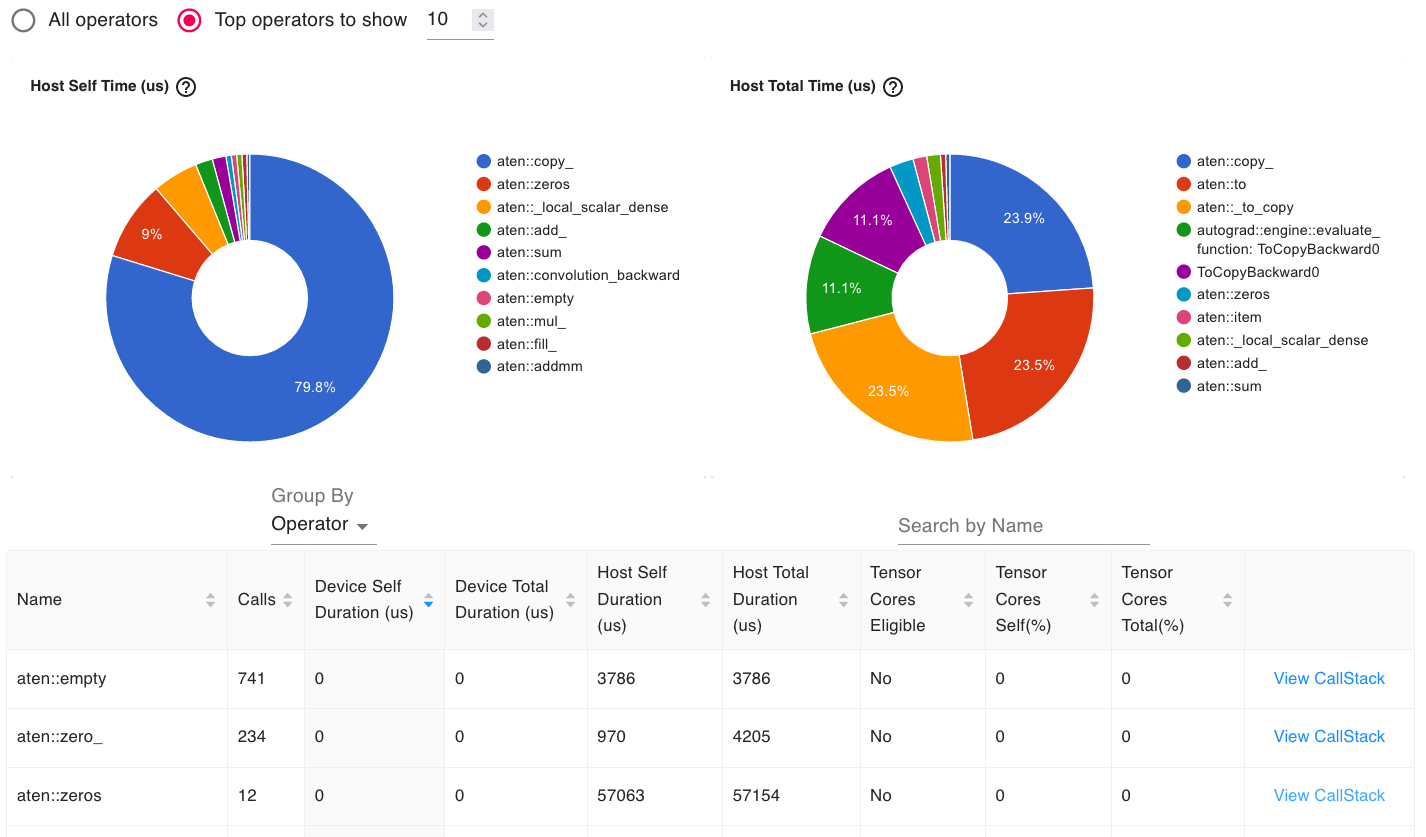
\includegraphics[width=0.9\textwidth]{./assets/scap_gtx1080_profiler-torch_batch-size-64_14650758_operator-view}
    \end{figure}
    \end{center}
\end{frame}

\begin{frame}{Operator View}
    \vspace{-1em}
\begin{center}
    \begin{figure}
        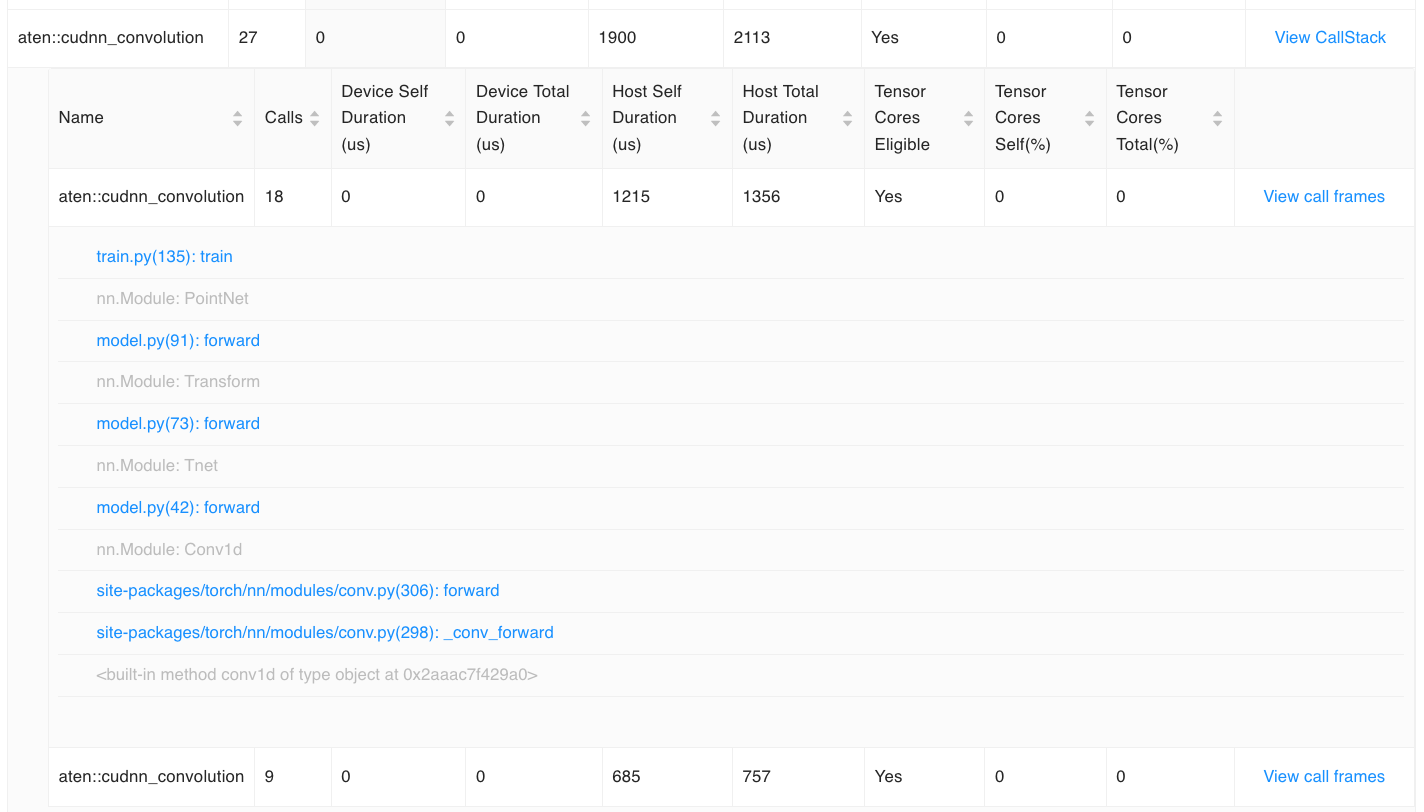
\includegraphics[width=0.9\textwidth]{./assets/scap_gtx1080_profiler-torch_batch-size-64_14650758_operator-view-details}
    \end{figure}
    \end{center}
\end{frame}

\begin{frame}{GPU Kernel View}
    \vspace{-1em}
\begin{center}
    \begin{figure}
        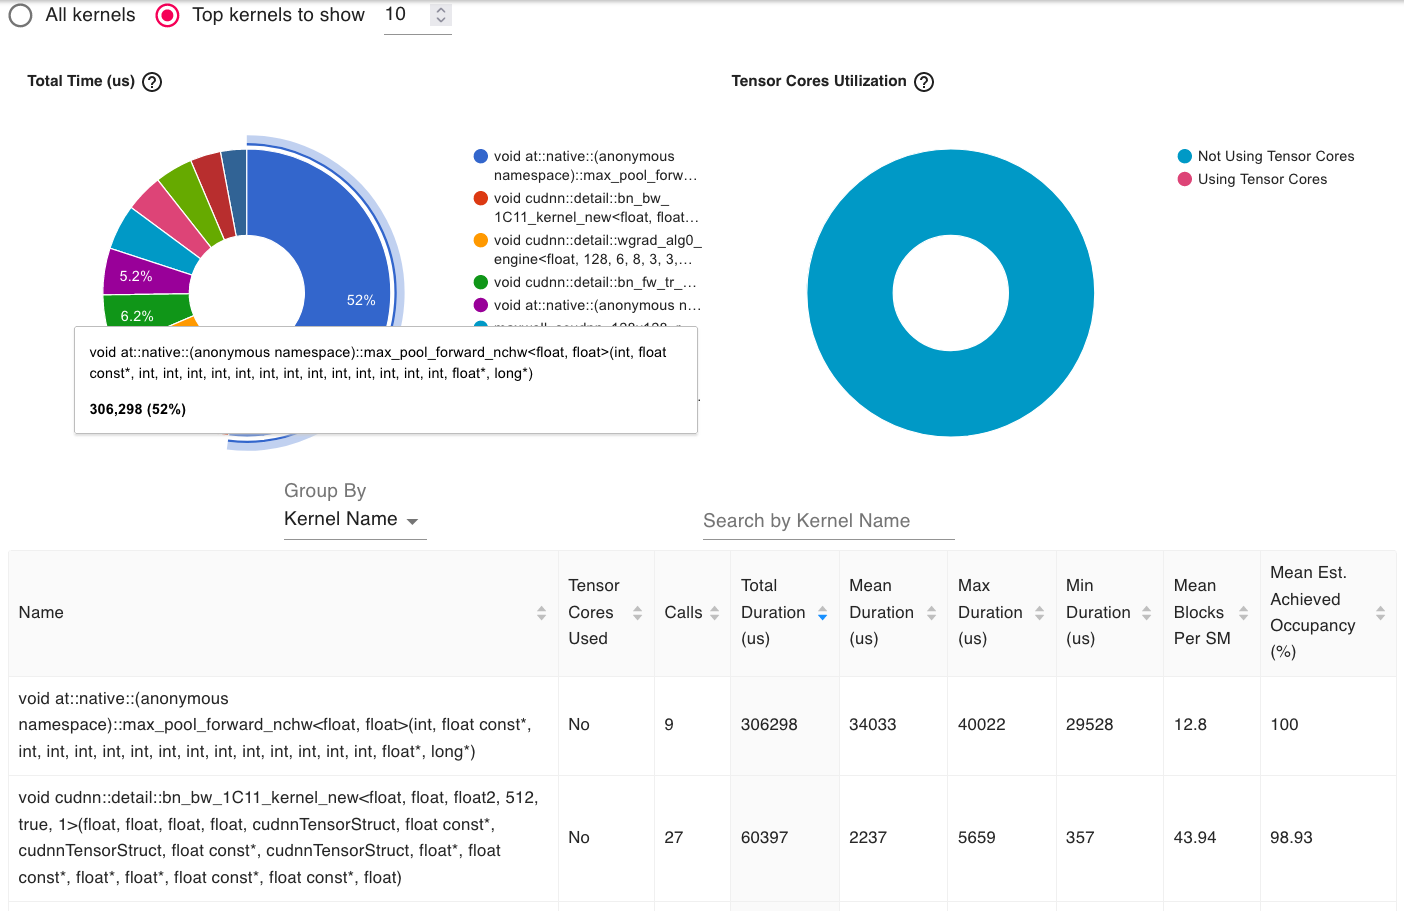
\includegraphics[width=0.9\textwidth]{./assets/scap_gtx1080_profiler-torch_batch-size-64_14650758_gpu-kernel-view}
    \end{figure}
    \end{center}
\end{frame}

\begin{frame}{Memory View}
    \vspace{-1em}
\begin{center}
    \begin{figure}
        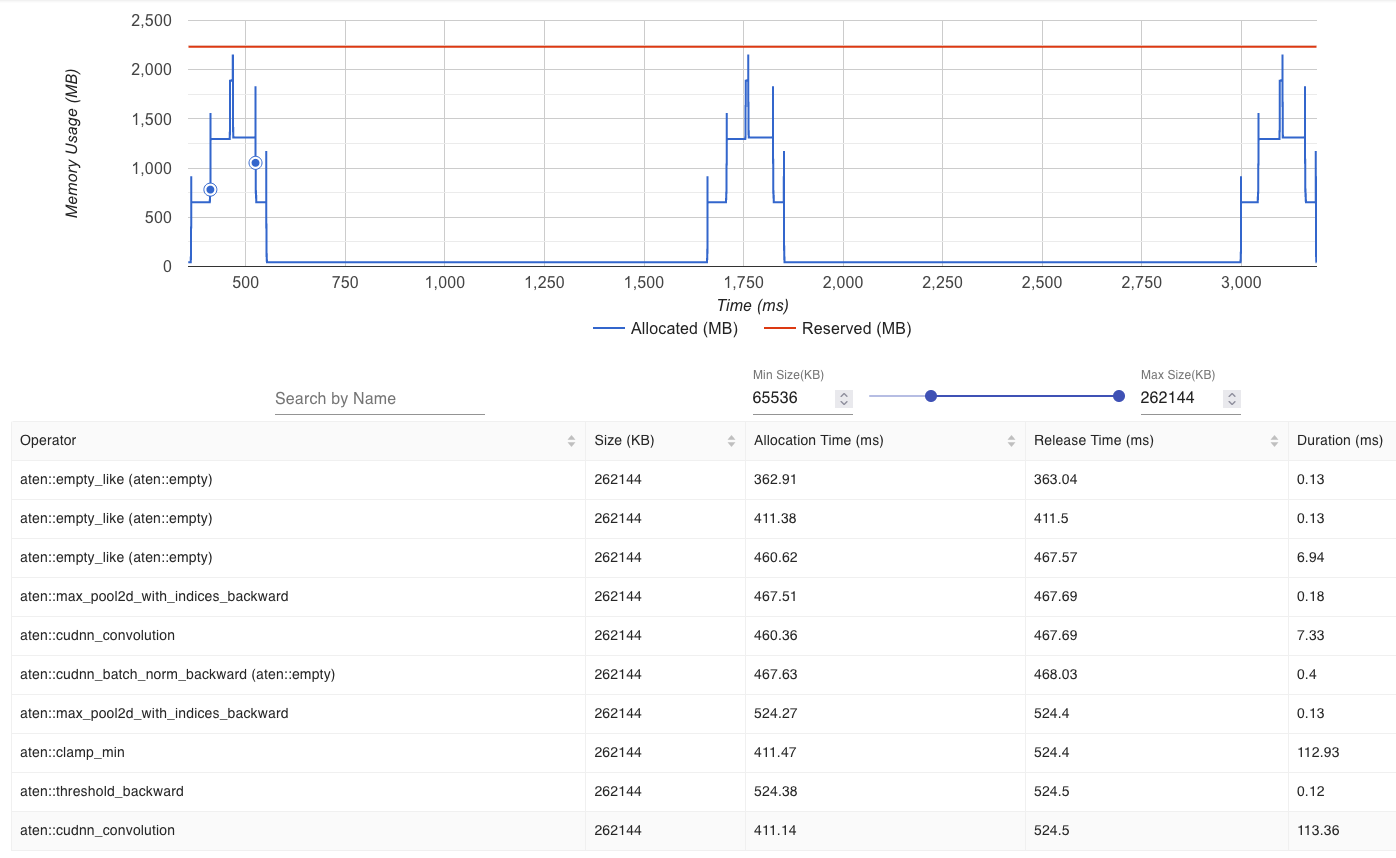
\includegraphics[width=0.85\textwidth]{./assets/scap_gtx1080_profiler-torch_batch-size-64_14650758_memory-view}
    \end{figure}
    \end{center}
\end{frame}

\begin{frame}{Module View}
    \vspace{-1em}
\begin{center}
    \begin{figure}
        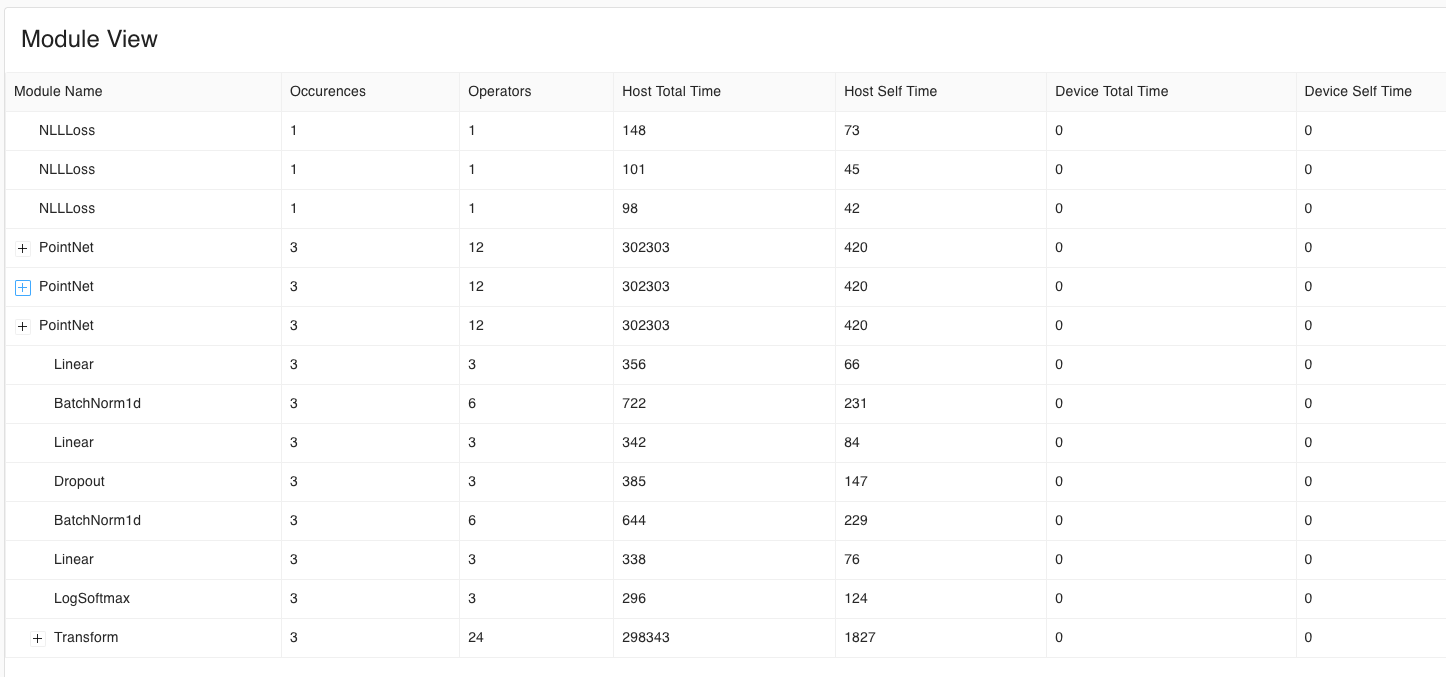
\includegraphics[width=1\textwidth]{./assets/scap_gtx1080_profiler-torch_batch-size-64_14650758_module-view}
    \end{figure}
    \end{center}
\end{frame}

\backupend

\end{document}
